\documentclass[12pt]{article}
\usepackage[papersize={8cm,14cm},margin={.5cm,.5cm}]{geometry}
\usepackage{common}
\usepackage{amssymb}
\begin{document}
\small
\begin{problem}[widest=10]
\item[10.] 圖(十)為兩正方形 $ABCD$、$BPQR$ 重疊的情形,其中 $R$ 點在 $\overline{AD}$ 上,$\overline{CD}$ 與 $\overline{QR}$ 相交於 $S$ 點。若兩正方形 $ABCD$、$BPQR$ 的面積分別為 $16$、$25$,則四邊形 $RBCS$ 的面積為何?
  \begin{figure}[ht]
    \centering
    \vspace*{-1ex}
    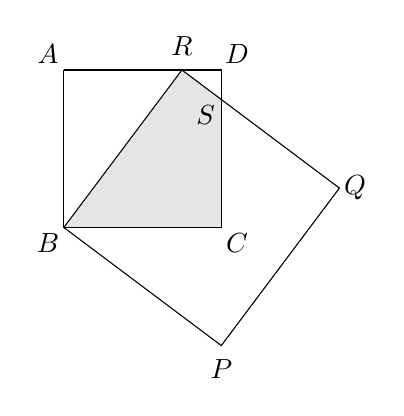
\begin{tikzpicture}
      \fill[black!10] (0,0) -- (1.5,2) -- (2,1.625) -- (2,0) -- (0,0);
      \draw (0,2) -- (0,0) -- (2,0) -- (2,2) -- (0,2);
      \draw (0,0) -- (1.5,2) -- (3.5,.5) -- (2,-1.5) -- (0,0);
      \node at (-.2,2.2) {$A$};
      \node at (-.2,-.2) {$B$};
      \node at (2.2,-.2) {$C$};
      \node at (2.2,2.2) {$D$};
      \node at (2,-1.8) {$P$};
      \node at (3.7,.5) {$Q$};
      \node at (1.5,2.3) {$R$};
      \node at (1.8,1.425) {$S$};
    \end{tikzpicture}
    \vspace*{-1ex}
    \caption*{圖(十)}
    \vspace*{-2ex}
  \end{figure}
  \begin{choices}
    \item $8$
    \item $\fraction{17}{2}$
    \item $\fraction{28}{3}$
    \item $\fraction{77}{8}$
  \end{choices}
\end{problem}
\end{document}
